% \documentclass[12pt]{article}%
% \usepackage{amsfonts}
% \usepackage{fancyhdr}
% \usepackage{comment}
% \usepackage[a4paper, top=2.5cm, bottom=2.5cm, left=2.2cm, right=2.2cm]%
% {geometry}
% \usepackage{times}
% \usepackage{amsmath}
% \usepackage{changepage}
% \usepackage{amssymb}

\documentclass[a4paper]{article}
\usepackage[margin=1in]{geometry}
\usepackage{graphicx}
\usepackage{indentfirst}
\usepackage{subcaption,multicol}
\usepackage{caption}
\setlength{\parindent}{2em}
\usepackage{physics} % provides lots of nice features and commands often used in physics, it 
\usepackage{siunitx} % typesets numbers with units very nicely
\usepackage{enumerate} % allows us to customize our lists
\usepackage{soul,color} % for revision
\usepackage{mathtools}

% \setcounter{MaxMatrixCols}{30}
% \newtheorem{theorem}{Theorem}
% \newtheorem{acknowledgement}[theorem]{Acknowledgement}
% \newtheorem{algorithm}[theorem]{Algorithm}
% \newtheorem{axiom}{Axiom}
% \newtheorem{case}[theorem]{Case}
% \newtheorem{claim}[theorem]{Claim}
% \newtheorem{conclusion}[theorem]{Conclusion}
% \newtheorem{condition}[theorem]{Condition}
% \newtheorem{conjecture}[theorem]{Conjecture}
% \newtheorem{corollary}[theorem]{Corollary}
% \newtheorem{criterion}[theorem]{Criterion}
% \newtheorem{definition}[theorem]{Definition}
% \newtheorem{example}[theorem]{Example}
% \newtheorem{exercise}[theorem]{Exercise}
% \newtheorem{lemma}[theorem]{Lemma}
% \newtheorem{notation}[theorem]{Notation}
% \newtheorem{problem}[theorem]{Problem}
% \newtheorem{proposition}[theorem]{Proposition}
% \newtheorem{remark}[theorem]{Remark}
% \newtheorem{solution}[theorem]{Solution}
% \newtheorem{summary}[theorem]{Summary}
% \newenvironment{proof}[1][Proof]{\textbf{#1.} }{\ \rule{0.5em}{0.5em}}

% \newcommand{\Q}{\mathbb{Q}}
% \newcommand{\R}{\mathbb{R}}
% \newcommand{\C}{\mathbb{C}}
% \newcommand{\Z}{\mathbb{Z}}

\begin{document}
	
	\title{Wireless Communication System Simulation}
	\author{Yu Liu, Bohan Zhang, Xianjun Mao}
	\date{\today}
	\maketitle
	
	\section{Introduction}
	
	In this course project, we simulated a wireless communication system which is closed to IEEE 802.11n standard based on MATLAB. Figure \ref{fig:ofdm_general} shows the structure of the simulated system. Moreover, data is collected from lab to estimate the channel statistically, which provides the simulation a model for real life propagation. In our project, the simulation features following elements:
	
	\begin{itemize}
		\item Channel Modelling 
		
		\subitem The channel is characterized with Power Delay Plan (PDP), and coherence bandwidth;
		\subitem Both narrowband and wideband model are extracted statistically from the lab data;
		
		\item OFDM communication system
		\subitem Additive White Gaussian Noise (AWGN) is considered in the channel;
		\subitem Channel estimation is implemented with Zero Forcing method;
		\subitem Synchronisation including frequency acquisition and time acquisition is implemented with preambles;
		\subitem Frequency tracking is implemented with 4 sub-carriers chosen as pilots carriers;
		
		\item SIMO simulation
		\subitem SIMO channels are characterized by beamforming. Spatial correlation and statistical model are extracted from measurement;
		\subitem SIMO OFDM communication system is simulated. The performance is compared with the corresponding SISO system;
	\end{itemize}
	
	The rest of the report is organised as following: Section 2 gives a brief introduction of the channel measurement and simulation settings; Section 3 introduce our channel modelling result; Section 4 mainly describes the whole OFDM communication system, with details on the synchronisation performance; Section 5 shows the simulation of SIMO system, whose performance is compared with the SISO system. Section 6 concludes the project by summarizing the simulation results. 
	
	\begin{figure}[ht]  
		\centering
		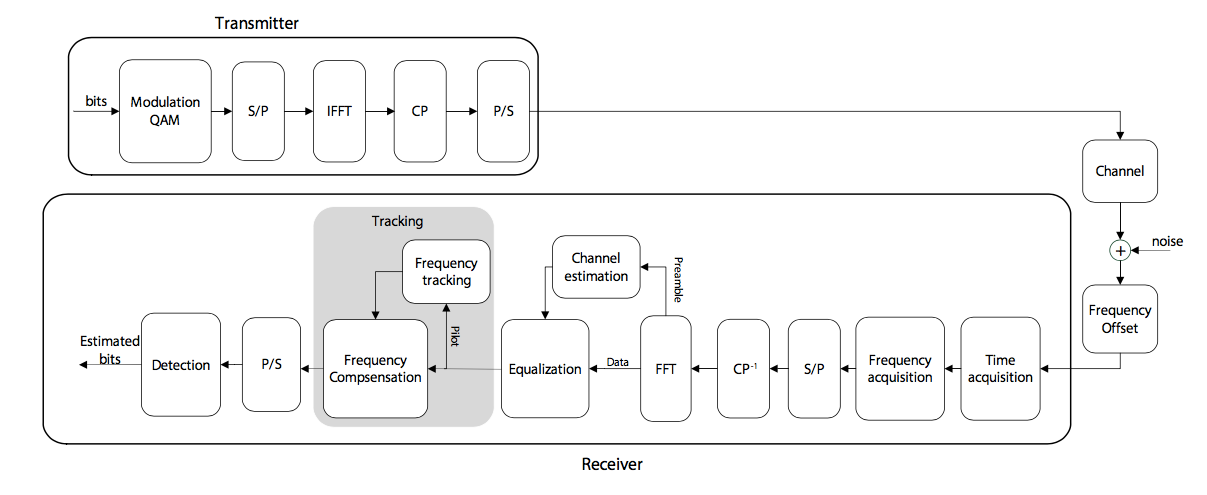
\includegraphics[width=0.9\linewidth]{figures/OFDM_general.png}
		\caption{Block diagram of OFDM communication system}
		\label{fig:ofdm_general}
	\end{figure}
	
	\section{Channel Measurement}
	
	During the channel measurement campaign, a 3D automatic positioning device is used to produce RX positions based on the placed TX. With the help of control software, the positions of RX are defined on a 3D grid, the each position means a channel acquisition is made. Finally, resulted in a construction of a virtual antenna array in a local area. In addition, two scenarios- Line of sight and Non Line Sight are considered in measurement campaign.
	
	In this project, a 10x10x10 virtual antenna array has 1000 positions separated by 2cm. For each position, the $H(f)$ $( $frequency response of channel transfer function$)$ is measured with a 200 MHz bandwidth and 400 KHz frequency resolution. In the next section, narrowband and wideband channel models will be established from these data for two scenarios.
	
	\section{SISO Communication}
	\subsection{Channel model}
	\subsubsection{Narrowband and Wideband}
	
	The narrowband and wideband is distinguished by whether the sampling frequency $f_s$ is larger than the coherence bandwidth $\Delta f_c$ or not. 
	
	\paragraph{Narrowband} For narrowband signal, the sampling frequency $f_s$ is much smaller than the coherence bandwidth $\Delta f_c$, which also means the sampling period $T_s$ is larger than the delay spread $\Delta_s$. This results leads to the effect that in time domain, the multi-path component(MPC) cannot be discriminated, which sums to one single tap for the impulse response $h(t)$ of the channel, the equation for it is showed in Eq \ref{eq:narrow0}. Fig.\ref{fig:ht_LOS} and Fig. \ref{fig:ht_NLOS} shows the channel transfer function amplitude in dB in the XY plane.
	
	\begin{align} 
		\begin{split}
			h(\vec{r}) = \sum_{i=1}^{N} a_i e^{j\phi_i}e^{-j\vec{\beta_i}\vec{r}}
		\end{split}
		\label{eq:narrow0}
	\end{align}
	
    \begin{figure}[h]
		\begin{minipage}[t]{0.5\linewidth}
			\centering
			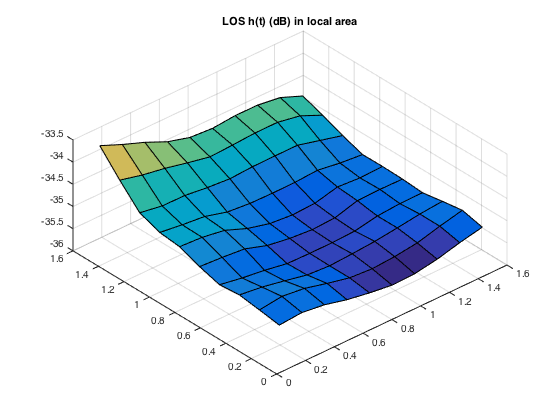
\includegraphics[scale=0.4]{figures/LOS_ht_LA.png}
            \vspace{-0.2cm}
            \centering
            \caption{LOS $|h(t)|$ (dB) in XY plane}
            \label{fig:ht_LOS}
		\end{minipage}
		\begin{minipage}[t]{0.5\linewidth}
			\centering
			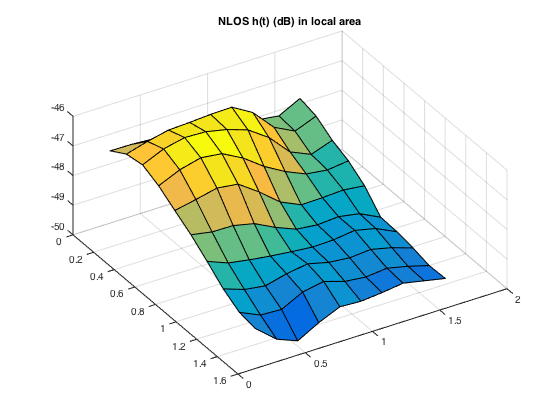
\includegraphics[scale=0.4]{figures/NLOS_ht_LA.png}
            \vspace{-0.2cm}
            \centering
            \caption{NLOS $|h(t)|$ (dB) in XY plane}
            \label{fig:ht_NLOS}
		\end{minipage}
	\end{figure}
    
	\paragraph{Wideband} For narrowband signal, the sampling frequency $f_s$ is much larger than the coherence bandwidth $\Delta f_c$, which also means the sampling period $T_s$ is smaller than the delay spread $\Delta_s$. This results leads to the effect that in time domain, the multi-path component(MPC) can be discriminated with certain number of taps. Eq. \ref{eq:wide0} shows the impulse response based on the wideband channel.
	
    \begin{figure}[h]
		\begin{minipage}[t]{0.5\linewidth}
			\centering
			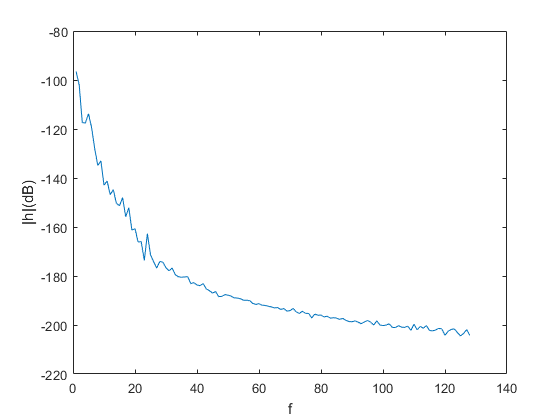
\includegraphics[scale=0.5]{lab1/PDP_Los.png}
			\vspace{-0.5cm}
			\centering
			\subcaption{LOS}
		\end{minipage}
		\begin{minipage}[t]{0.5\linewidth}
			\centering
			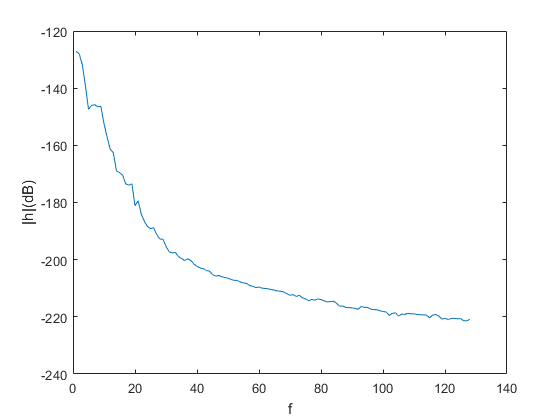
\includegraphics[scale=0.5]{lab1/PDP_NLos.png}
			\vspace{-0.5cm}
			\centering
			\subcaption{NLOS}
		\end{minipage}
		\caption{The PDP of two scenarios (200Mhz)}
        \label{fig:pdp200}
	\end{figure}
    
	\begin{align} 
		\begin{split}
			\hat{h}(n) = \sum_{i=1}^{N} a_i e^{j\phi_i}e^{-j\vec{\beta_i}\vec{r}}\delta(n\Delta\tau-\tau_i)
		\end{split}
		\label{eq:wide0}
	\end{align}
	
	\subsubsection{Distribution of the tap}
	\noindent
	Relied on measured data, the impulse response is calculated in Matlab. A function $ifft3d$ is introduced to extract channel frequency response and compute ifft at each position. After calculating impulse response, the next step is to extract the Power Delay Profile$($PDP$)$, which is mean received power in function of delay. Under the \textit{N-waves Model}, and with the assumption of \textit{Uncorrelated Scattering}. The channel is \textbf{Wide Sense Stationary} in frequency. Say the frequency correlation $R(\Delta f)$ and PDP $P(\tau)$ is a Fourier transform pair.
	
	The ifft size keeps constant, therefore the size of impulse response at each point is still 501. In oder to eliminate the effect of small-scale fading As seen in Eq .3,  the N is set to 1000 to average all position. Power Delay Profile in LOS and NLOS scenarios are depicted in Figure.2, follows an exponential decay, the time dispersion of the channel can be observed.
	
	\begin{align} 
		PDP(n)=\frac{1}{N}\sum_i^N|h_i(n)|^{2}
	\end{align}
	where the $i$ is position index.
	
	The delay spread $\sigma_\tau$ characterizes the PDP duration, which also indicates the spread of the energy. It can be calculated directly from the PDP of the signal as showed in Eq. \ref{eq:delayspread}. Coherence bandwidth $f_c$ can be easily derived from delay spread following $f_c = \frac{1}{2 \pi \sigma_\tau}$ In this part, the delay spread $\sigma_\tau$, and ${\Delta}f_c$ is calculated and results is shown in table 1. 
    
    \begin{align} 
		\begin{split}
			\sigma_\tau = \sqrt{\frac{1}{P_T}\int_0^{\infty} \tau^2P(\tau)d\tau - \tau_m^2 }
		\end{split}
		\label{eq:delayspread}
	\end{align}
	
    The channel coherence bandwidth  ${\Delta}f_c$ is used to distinguish if a certain signal with bandwidth $B$ will experience flat fading or frequency selective fading.
    
	% TODO: the title of figure is erased by white, which is weired, cut it or fix the title [MAO]
	When the interest bandwidth reduce from 200MHz to 20 MHz, the window is needed to achieve the bandwidth reduce. In this section, two types of windows is established: rectangular and non-rectangular$($tukey$)$ window. The tukey window is designed by function $tukeywin(L,r)$. We set last 5 percent of the samples equal to parts of a cosine seen in Figure.3.  
	\begin{figure}
		\centering
		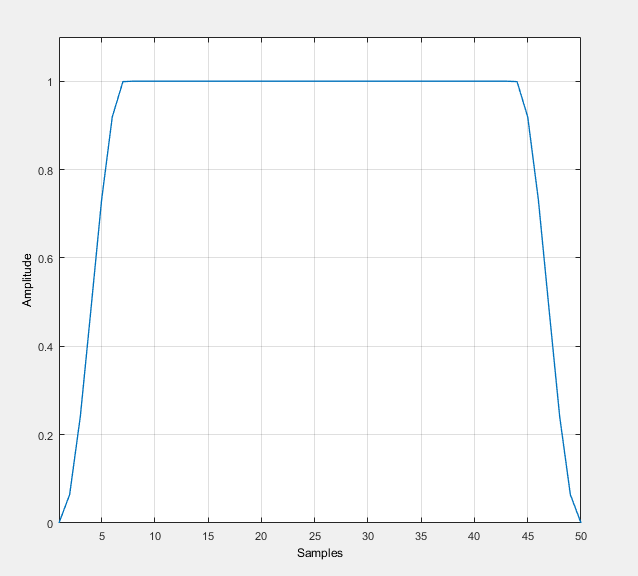
\includegraphics[scale=0.4]{lab1/tukey__2_.png}
		\vspace{-0.2cm}
		\centering
		\caption{The Tuckey window}
		\label{fig:tuckey_window}
	\end{figure}
	
	Under above situation, four new PDP are depicted in  Figure.4 and 5, lead to four groups of delay spread and coherence bandwidth, see in table 2. 
	\begin{figure}[hbtp]
		\begin{minipage}[t]{0.5\linewidth}
			\centering
			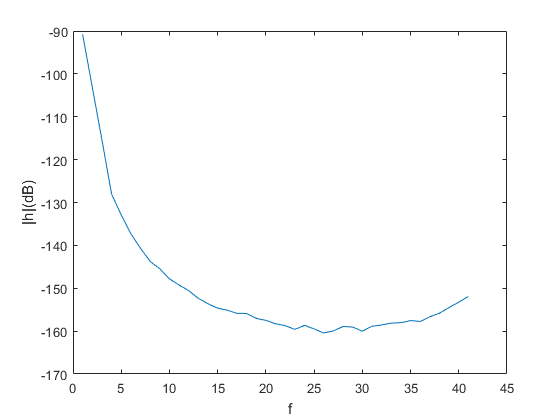
\includegraphics[scale=0.5]{lab1/PDP_LOS_rec.png}
			\vspace{-0.5cm}
			\centering
			\subcaption{LOS}
		\end{minipage}
		\begin{minipage}[t]{0.5\linewidth}
			\centering
			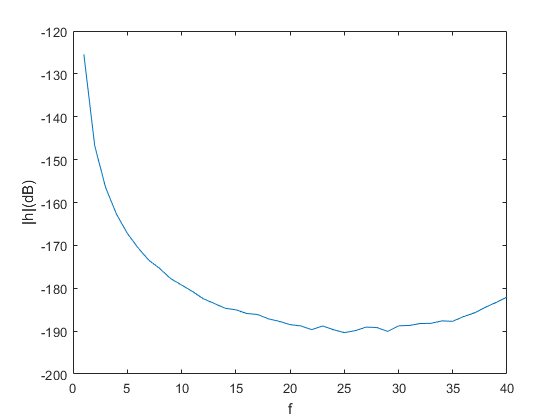
\includegraphics[scale=0.5]{lab1/PDP_NLOS_rec.png}
			\vspace{-0.5cm}
			\centering
			\subcaption{NLOS}
		\end{minipage}
		\caption{The PDP of two scenarios (rectangle window)}
        \label{fig:rec_win_PDP}
	\end{figure}
	\begin{figure}[hbtp]
		\begin{minipage}[t]{0.5\linewidth}
			\centering
			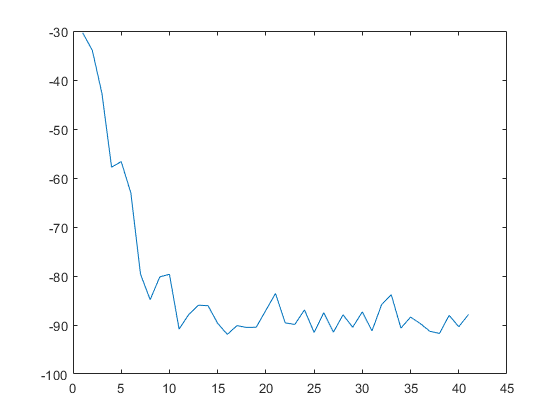
\includegraphics[scale=0.5]{lab1/PDP_LOS_tuck.png}
			\vspace{-0.5cm}
			\centering
			\subcaption{LOS}
		\end{minipage}
		\begin{minipage}[t]{0.5\linewidth}
			\centering
			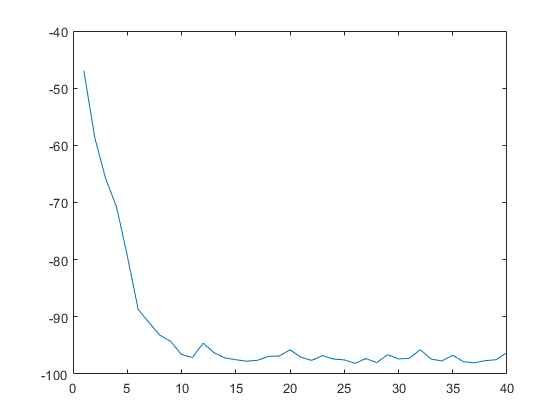
\includegraphics[scale=0.5]{lab1/PDP_NLOS_tuck.png}
			\vspace{-0.5cm}
			\centering
			\subcaption{NLOS}
		\end{minipage}
		\caption{The PDP of two scenarios (tuckey window)}
		\label{fig:tuckey_PDP}
	\end{figure}
	
    	\begin{table}[h]
		\centering 
		\begin{tabular}{lcc}
			\hline
			Modes &LOS &NLOS \\
			\hline 
			\centering{ $\sigma_{\tau}$}  &1.4778e-8 &2.0681e-8 \\ 
			\hline 
			\centering{  ${\Delta}f_c($Hz$)$}  &11088386.9204 &7695686.3627 
			\\  \hline 
		\end{tabular}
		\caption{the delay spread and coherence frequency for 200MHz}
		\label{tb:ds_rec}
	\end{table}
	
	\begin{table}[h]
		\centering 
		\begin{tabular}{lcccc}
			\hline
			Modes &LOS(rec) &LOS(tuckey) &NLOS(rec) &NLOS(tuckey)\\
			\hline 
			\centering{ $\sigma_{\tau}$}  &1.411e-7 &3.0183e-08 &1.7334e-07 &2.8560e-08\\ 
			\hline 
			\centering{  ${\Delta}f_c(Hz)$}  & 1127663.5984 &5273077.7274 &918154.0045 &5572605.7692
			\\  \hline 
		\end{tabular}
		\caption{the delay spread and coherence frequency for filtered signal}
		\label{tb:coherence_f}
	\end{table}

	\vspace*{+5mm}	
	\noindent\fbox{%
		\parbox{\textwidth}{%
			\paragraph{Discussions}
			\begin{itemize}
				\item Extract the channel frequency response, calculate the impulse response at each position.
				\item Observe the effect of limited bandwidth, and fix this problem
				\subitem Originally the data is collected by scanning through \textit{200Mhz} with 500 points. If we limit the frequency to \textit{20Mhz} by directly clipping the data it will cause aliasing in time domain, due to the discontinuity in frequency domain. The problem can be observed in Fig.4. The solution is to filter the clipped signal in frequency domain with a end-diminish filter (In this project, we choose Tuckey window, see Fig. \ref{fig:tuckey_window}). After filtering in frequency domain, the signal in time domain can be seen in Fig. \ref{fig:tuckey_PDP}.
				\item Extract the PDP, and calculate the delay spread and confirm the exponential decay.
				\subitem The PDP figure refers to Fig.\ref{fig:pdp200} , the delay spread refers to Table. \ref{tb:coherence_f} \\
				\textbf{It is also worth mentioning that, as the measuring equipment cannot satisfy the whole 200MHz scale. It also works as a low-pass filter. Which will introduce certain delay in the PDP. So we have to clip it from the first max value.}
				\item Evaluate the coherence bandwidth;
				\subitem The coherence bandwidth $f_c$ is showed in Table \ref{tb:coherence_f}. From the table it can be observed: (i) LOS gives a higher coherence bandwidth. This is probably due to the line of sight wave, which reduces the effect of multiple path. (ii) Tuckey window gives a better performance compared to the rectangular window. Since the rectangular window would cause discontinuity at the boarder in the frequency domain, contributing to unwanted response in the time domain, which also leads to longer delay time. 
                
                \item Reduce the bandwidth to 20 MHz using a rectangular and non-rectangular window. Interpret the impact on the impulse response (Power Delay Profile, Delay Spread, Coherence Bandwidth).
                \subitem From Table \ref{tb:coherence_f} and Fig. \ref{fig:rec_win_PDP}, we can observe that using rectangular window will cause unwanted response in time domain, while Tuckey window filtering does not have this problem. Furthermore, applying rectangular window will reduce the coherence bandwidth significantly. The reason for these effects is briefly analyzed in last point.
			\end{itemize}
		}%
	}
	

	\subsubsection{Statistical Model}
	
	For a given wireless communication channels, it can be seen as a set of incident plane waves in a local area $A$. The transfer function of the channels could be calculated through Eq. \ref{eq:narrow0} and Eq. \ref{eq:wide0}. However, practically, as the environment including the interactive objects(OIs) are constantly changing, it is hard to model the channel characteristics. Instead, we model the channel statistically. 
	
	For narrowband NLOS situation, the deterministic model for the channel transfer function is:
	\begin{align} 
		\begin{split}
			h = A e^{j\Phi}
		\end{split}
		\label{eq:stat_narrow_NLOS}
	\end{align}
    
    where the $\phi$ is a random variable with uniform distribution and $A$ follows Rayleigh distribution. However,there is another case when channel is LOS. Due to the different propagation characteristic, the amplitude of the impulse response is following Rice distribution and can be written as Eq. \ref{eq:stat_wide_LOS}.
	\begin{align} 
		\begin{split}
			h = \sqrt[]{\frac{K}{K+1}}e^{j\Phi}+\sqrt[]{\frac{1}{K+1}}A e^{j\Phi}
		\end{split}
		\label{eq:stat_wide_LOS}
	\end{align}
    
   Where the K is the Rice factor. \textbf{It is possible to show that the Rician factor $K$ gives the relative power of the LOS component compare to the mean power of the multipath. With growing $K$ the distribution becomes more and more tight, the LOS component becomes more and more dominant}. As mentioned in previous section, the wideband models take into account time dispersion,  each tap in wideband is associated a stochastic model and also obey same distribution as the narrowband.
   
   In this project, first step is to bulid a narrowband model for LOS and NLOS. In order to satisfied the narrowband (only one tap consist of a bunch  of wave), we sum all points at each  position, get 1 taps at one position. Then use the toolbox dfittool in matlab and data to fit the Rice and Rayleigh distribution. The parameter covariance of  Rayleigh distribution for NLOS and LOS are 
2.5e-10 and 3.09e-9, verify the statistical law in NLOS. The same verify also exist in  LOS situation.
   After verify the distribution law, we can calculate the parameters of different distribution, the Rice factor K in narrowand is shown in table.\ref{tb:k in narrow}.
   
   
 \begin{table}[h]
		\centering 
		\begin{tabular}{lcccc}
			\hline
			Models &Narrowband LOS \\
			\hline 
			\centering{ $k$}  &1.8294 \\ 
			\hline 
		\end{tabular}
		\caption{the Rice factor K in narrowband}
		\label{tb:k in narrow}
	\end{table}
	
	The second step is extended to the wideband model under 20MHz situation. For each tap in $h(t)$, we use all the 1000 points collected by the receiver matrix to fit the distribution. Same as the  computation for narrowband model, compare the parameter covariances of two distribution in NLOS and LOS at each tap, the NLOS has better "goodness" to fit the Rayleigh distribution. On the other hand, the LOS has better "goodness" to fit Rice distribution. The evolution of Rice factor K is shown in Table.4.
    
    
    \vspace*{+5mm}
	\noindent\fbox{%
		\parbox{\textwidth}{%
			\paragraph{Discussions}
			\begin{itemize}
				\item Build a narrowband model and verify the statistical distribution. Explain the Rice factor K.
				\subitem The narrowband model is built by sum up all the impulse response from all taps. Statistical distribution is acquired through the 1000 observations; As showed in Eq.\ref{eq:stat_narrow_NLOS}, when $K=0$, the Rice distribution is degraded to Rayleigh distribution. The Rice factor K is explained in the bold font part in above section.
				
				\item In the wideband case, for each tap, verify the statistical distribution law and calculate the parameters. Show the evolution of Rice factor K through the time delay.
				\subitem As explained in previous point, the rice factor $K$ indicates the dominance of the LOS component. We show the $K$ value of the first 6 taps in Table \ref{tb:kforwb}. From the table, we can observe that the factor K is quite high at the first few taps, and diminish to around 1 after the first few taps. This character maybe caused by the transmitter source character.
				
			\end{itemize}
		}%
	}
	
     \begin{table}[h]
		\centering 
		\begin{tabular}{lcccccc}
			\hline
			Taps &1 &2 &3 &4 &5 &6 \\
			\hline 
			\centering{ $K$}  &4.0055 &2.8696 &1.1078 &1.9071 &1.1713 &1.3041 \\ 
			\hline 
		\end{tabular}
		\caption{the Rice factor K in wideband}
		\label{tb:kforwb}
	\end{table}
    
    \begin{figure}
		\centering
		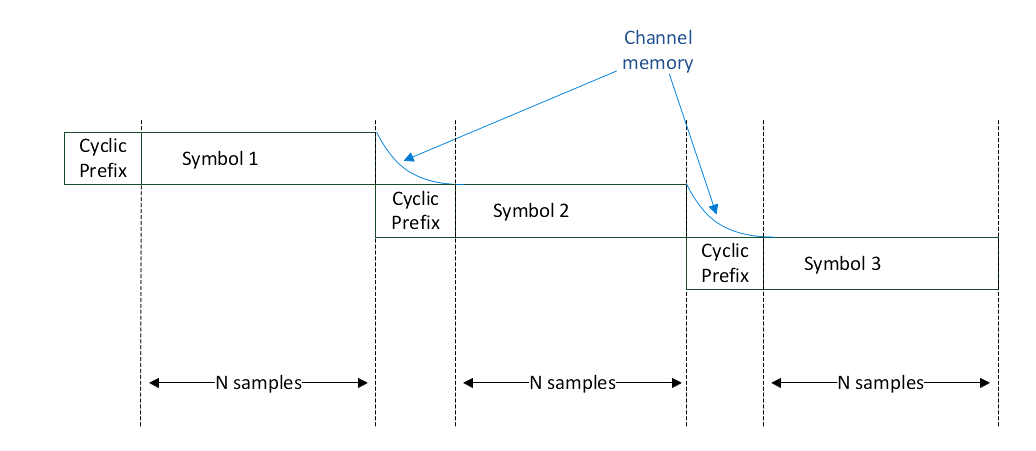
\includegraphics[scale=0.45]{figures/ibi_show.png}
		\vspace{-0.2cm}
		\centering
		\caption{Demonstration for CP effect on IBI}
		\label{fig:cpIBI}
	\end{figure} 
	
	\section{OFDM communication system}
	
	In this section we simulated a wireless communication system, from the transmitter to the receiver end. AWGN and MPC are considered in the channel. We utilized the channel statistical model acquired in Section 2 to simulate the MPC effect. The system structure is demonstrated in Fig. \ref{fig:ofdm_general}. The specification of the system in our project is showed in Table. \ref{tb:spec in system}
    
     \begin{table}[h]
		\centering 
		\begin{tabular}{lcccc}
			\hline	
            	\centering{ Length of signal}  &$L$ &1024*60 \\ 
			
			\centering{ Numer of subcarriers}  &N &64 \\ 
			 
			\centering{ CP Length}  &$L_{cp}$ &16 \\ 
		
            	\centering{ Bandwidth}  &B &20MHz \\ 
			 
            	\centering{ Carrier frquency}  &$f_c$ &2.35GHz\\ 
			\hline      
		\end{tabular}
		\caption{the specification  of OFDM system}
		\label{tb:spec in system}
	\end{table}
	
	%TODO: add a table indicating the parameters
	
	\subsection{Channel equalization}
	
	As Inter-symbol Inference(ISI) occurs when the multiple delayed replicas of the transmitted signal are received in case of a multi-path channel. Each replica creates a interference between successive symbols. 
	
	When no ISI is considered, matched filter at the receiver side can maximize the SNR. An equalizer is used to mitigate ISI caused by the multi-path channel. In this project, we use the Zero-forcing equalizer, which is simply the inverts of the channel:
	
	\begin{align} 
		\begin{split}
			F_{ZF} = (H^H \cdot H) ^{-1} \cdot H^H
		\end{split}
		\label{eq:ZF}
	\end{align}
	
	ZF equalizer suffers from the channel because it amplifies the noise significantly where the channel attenuation is high. 
    
  Time filter is complex and not efficient for long channel, So it is possible to implement the equalizer with scalar multiplications in the frequency domain by using some tips.
Therefore, the OFDM is used to achieve the equalization, transmit independent symbols on orthogonal sub-carriers. In Eq. \ref{eq:tdconv} , the convolution product in time domain is converted to more simple multiplication in freq domain at the receiver. However, the problem is that the relation works when the $s(n)$ is periodic, if not, we cannot implement the equalizer in freq domain.

\begin{align} 
		\begin{split}
			r = \sum_{m=0}^{L-1}h_mp_{n-m} + z_n
		\end{split}
		\label{eq:tdconv}
	\end{align}

 Thus, add the Cyclic prefix in front of the each data block,is introduced to help the periodicity created. Because the CP added, the blocks interference only take place between the last sample of one block and CP of the next block. At the receiver , the interference will be canceled, seen in Fig.\ref{fig:cpIBI}
 
 In this section, OFDM transmitter and receiver is implemented with following features:
 
  1) Transmitter: generate a random bits stream $($the length of bit stream is 60*1024 $)$ and adding preambles for channel equalization and synchronization use;  The modulated symbols$($64-QAM$)$ is converted in a sequence of 64-point block by using $reshape$ function, then we get 64 sub-carriers. After ifft, 16-point CP is added to each block, the new length of block is 80 points. 
  
  2) Noise: in order to simulate the reality and observe the BER. It is necessary to add white noise before receiver. There the range of  EbN0 $($dB$)$ is set to $[$-50 , 50$]$. The corresponding power of different noise can be calculated. 
  
  3) Receiver:  built with channel estimation, time shifting and frequency offset acquisition, and frequency tracking. The removal of CP is finished at the receiver.  By using  $demapping$ function, generate the estimated bits. 
  
   Until this step, we can simulate and verify something without channel added. The constellation of received signal is shown in Fig.\ref{fig:cpICI}. There exist a significant difference between two situations, which verify the importance of CP. The BER performance without channel in the presence of noise can also be observed in Fig.\ref{fig:ber_awgn_nochannel}
   
   4) Add the channel: After above three steps finished, the channel model from last section is added to the whole system behind FFT, the equalization is implemented by Zero- forcing equalizer.
   
   Finally, the BER performance of system with channel is shown in Fig.\ref{fig:ber_awgn_only}.

      \begin{figure}
		\centering
		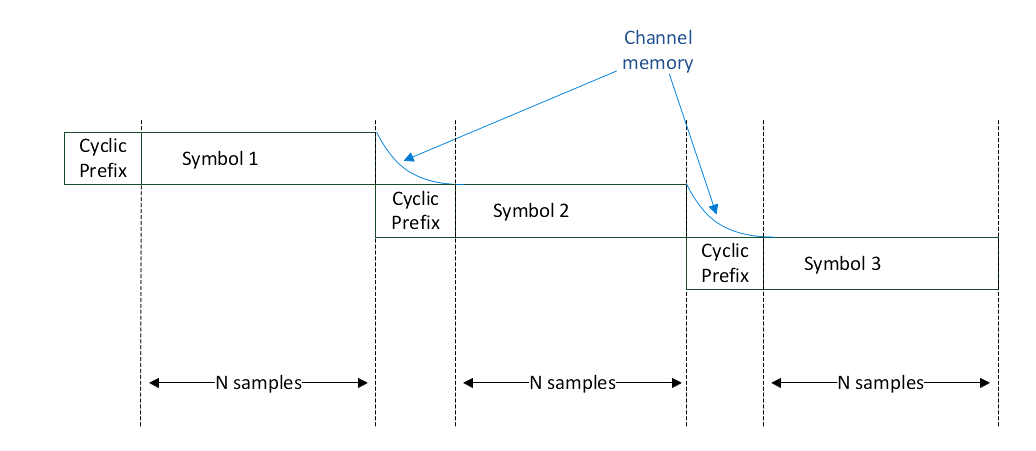
\includegraphics[scale=0.45]{figures/ibi_show.png}
		\vspace{-0.2cm}
		\centering
		\caption{Demonstration for CP effect on IBI}
		\label{fig:cpIBI}
	\end{figure} 
    
        \begin{figure}
		\centering
		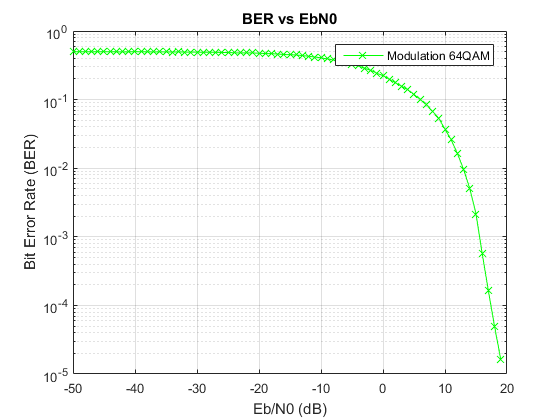
\includegraphics[scale=0.6]{figures/NoChannelBER.png}
		\vspace{-0.2cm}
		\centering
		\caption{BER vs EbN0 Channel unknown}
		\label{fig:ber_awgn_nochannel}
	\end{figure}
    
  
    
    \begin{figure}[hbtp]
		\begin{minipage}[t]{0.5\linewidth}
			\centering
			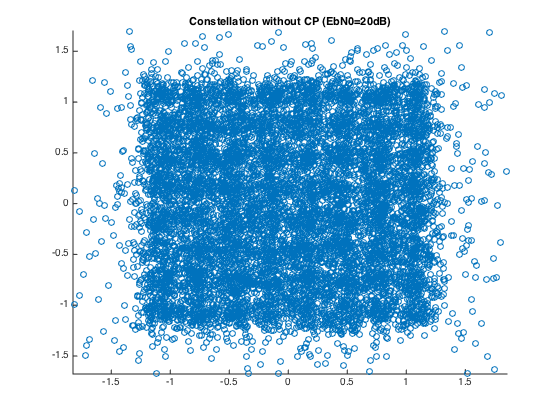
\includegraphics[scale=0.5]{figures/const_nocp.png}
			\vspace{-0.5cm}
			\centering
			\subcaption{Constellation of received signal (EbN0=20dB no CP)}
		\end{minipage}
		\begin{minipage}[t]{0.5\linewidth}
			\centering
			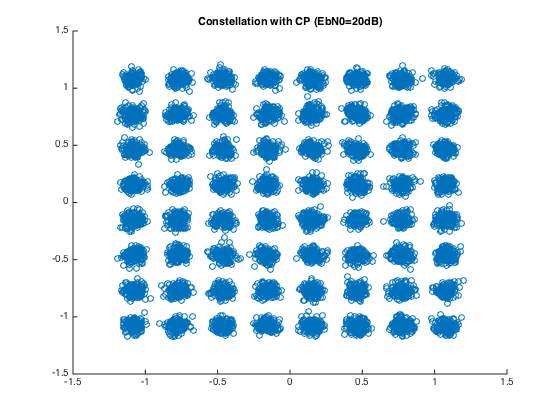
\includegraphics[scale=0.5]{figures/const_cp.png}
			\vspace{-0.5cm}
			\centering
			\subcaption{Constellation of received signal (EbN0=20dB avec CP)}
		\end{minipage}
		\caption{Verifying the CP effect on ICI}
		\label{fig:cpICI}
	\end{figure}
    
    \begin{figure}
		\centering
		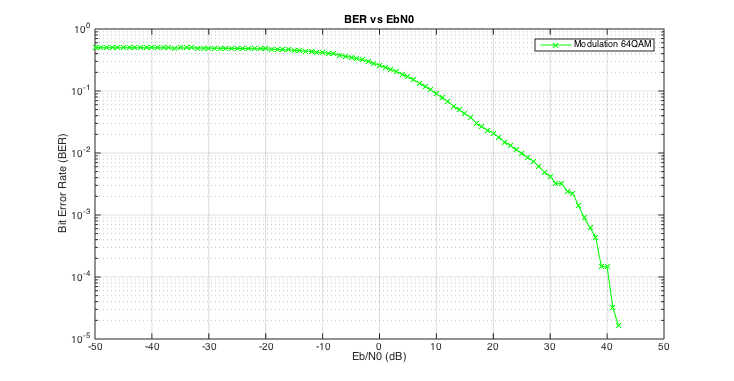
\includegraphics[scale=0.5]{figures/ber_ebno_awgn_only.png}
		\vspace{-0.2cm}
		\centering
		\caption{BER vs EbN0 (channel known for equalization)}
		\label{fig:ber_awgn_only}
	\end{figure}
 
	\vspace*{+5mm}
	
	\noindent\fbox{%
		\parbox{\textwidth}{%
			\paragraph{Discussions}
			\begin{itemize}
				\item Explain why the CP addition allows to restore orthogonality among sub-carriers. Verify that there is neither Inter-Carrier Interference nor Inter-Block Inference.
				\subitem The cyclic prefix (CP) is added to the head of each block by repeating the ending of block. The effect of CP is twofold: (i) By adding a $L_{CP}$ length CP, it can mitigate the channel memory corruption. See Fig.  (ii) By repeating the last few symbols, it makes the block periodic which ensures the orthogonality among the sub-carriers.
				Compare the result in Fig. \ref{fig:cpICI} we can observe that adding CP with appropriate length will mitigate the ICI effectively. Fig. \ref{fig:cpIBI} demonstrates that CP can solve the IBI problem by making enough room for the memory of channel (which also indicates that the length of CP should be at least longer than the expecting order of channel transfer function).
				
				\item Assess the BER performance of OFDM system in the presence of additive noise
				\subitem The BER performance of OFDM system is demonstrated in following figure. In the figure we can observe that the BER performance degraded with the increasing of AWGN.
				\item Apply the channel equalization to the signal. Suppose the channel is known by receiver.
				\subitem The channel equalization will work perfectly when the channel is known. The result can be seen in Fig. \ref{fig:ber_awgn_only}
				\item Discuss the impact of channel parameters on the choice of modulation parameters
				\subitem The channel parameters has deterministic impact on the choice modulation parameters: (i) If the sampling frequency $f_s$ is lower than the coherence bandwidth $\Delta f_c$, the channel can be fit as a narrowband model, MPC can hardly be distinguished. (ii) CP length should be larger than the delay spread $\sigma_t$, since the CP is added to mitigate the channel memory effect.(iii) Block size is depending on the number of sub-carriers and the CP length.
				\item Confirm that each sub-carrier is affected by a narrowband channel in our case.
				\subitem The wideband channel is represented by a 8-tap long impulse response $h(t)$ in the simulation. Across the channel, $h(t)$ is convoluted with the signal in time domain, which equivalent to multiplication with channel coefficient in each sub-carrier in frequency domain. In this way, it can also be seen as a narrowband channel in each sub-carrier.
				\item It worth mentioning that by keeping only one block and its CP is equivalent to multiplying a \textit{sinc} signal in the frequency domain. In practice bandwidth limiting is carried out by disabling several frequencies at the boarder.
			\end{itemize}
		}%
	}
	
    
    
	\subsection{Channel Estimation}
	
	As all the equalizer considered from the lecture is depending on the knowledge of the channel impulse response $h(t)$. Although we have established the NLOS and LOS channel response in previous section, the real $h(t)$ is unobservable directly in reality.Thus, a channel estimation becomes essential for the system. In this simulation, we build the channel estimation by applying a preamble sequence at the beginning of the data stream, seen in Fig.\ref{fig:preamble}. The content of the preamble is known both by the transmitter and the receiver.
    
    In order to satisfied the requirement, we generate a series data in freq domain firstly, ensure the same power as the data symbol. Then transform it to time domain and add in front of the bitstream to form the overall frame.
    At the receiver, the received overall frame should convert to parallel and remove CP, then use the FFT to generate freq domain signal. Meantime, extract the preamble part to finish the estimation for next equalization. Actually, the FFT of preamble is independent with symbol. In a world, it is impossible to extract the preamble in time domain and finish estimation at the beginning of receiver. The advantage of that is provide the convenience to compute the estimation in time domain.
    
    After implement the estimation, the channel error should be considered. The "NMSE" Eq.\ref{eq:NMSE} is always used to asses the accuracy. Based on the Eq.\ref{eq:estimation}, the numerator of NMSE is proportional to power of noise, so we can find the "NMSE" as a function of "SNR". The Fig.\ref{fig:NMSE0} shows the value of "NMSE" in different "SNR", follow a negative correlation.
    Finally, it is necessary to asses the BER performance under estimation by comparing it with BER performance without estimation, the result shown in the Fig.\ref{fig:es_or_not}.
    
    
      \begin{figure}
		\centering
		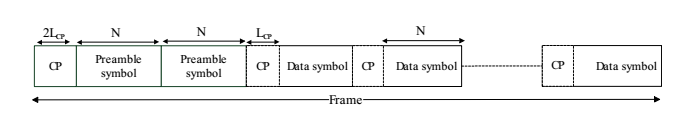
\includegraphics[scale=0.5]{figures/preamble.png}
		\vspace{-0.2cm}
		\centering
		\caption{Frame structure}
		\label{fig:preamble}
	\end{figure}
    
   \begin{align} 
					\begin{split}
						\ NMSE = \frac{\sum_{k} |\hat{H}{(k)}-H(k)|^2}               {\sum_{k} |H(k)|^2} 
					\end{split}
					\label{eq:NMSE}
				\end{align}
                
         \begin{align} 
					\begin{split}
						\ \hat{H}{(k)} =H(k)+ \frac{W(K)}{S(K)} 
					\end{split}
					\label{eq:estimation}
				\end{align}       
                
        \begin{figure}[hbtp]
		\begin{minipage}[t]{0.5\linewidth}
			\centering
			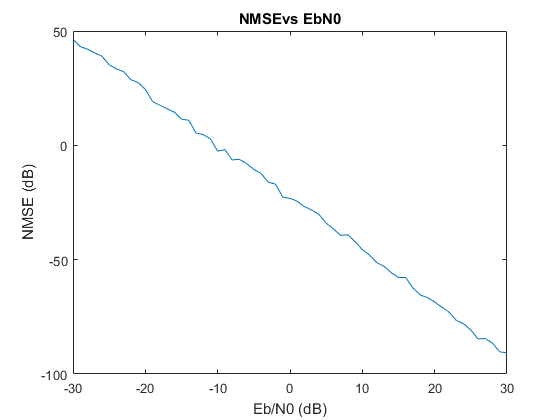
\includegraphics[scale=0.5]{figures/NMSE.png}
			\vspace{-0.3cm}
			\centering
			\caption{NMSE vs EbN0}
            \label{fig:NMSE0}
		\end{minipage}
		\begin{minipage}[t]{0.5\linewidth}
			\centering
			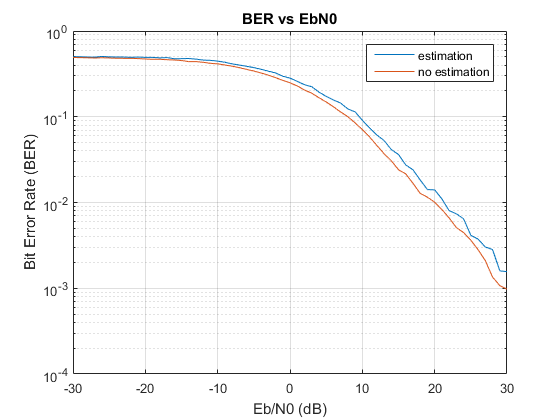
\includegraphics[scale=0.5]{figures/estimate_or_not.png}
			\vspace{-0.3cm}
			\centering
			\caption{The BER vs EbN0}
               \label{fig:es_or_not}
		\end{minipage}
		
		
	\end{figure}

	\vspace*{+5mm}
	
	\noindent\fbox{%
		\parbox{\textwidth}{%
			\paragraph{Discussions}
			\begin{itemize}
				\item Form the preamble and implement the channel estimation. Keep in mind that the power of the preamble should be equal to the power of the rest of the signal.
				\subitem It worth mention that the estimation error depends on the sequence of pilot symbols. Assuming $P$ is the pilot symbols. The estimated channel with ML is:
				
				\begin{align} 
					\begin{split}
						\hat{h} = h + (P^H \cdot P) ^{-1} \cdot P^{H} \cdot z
					\end{split}
					\label{eq:estimate}
				\end{align}
				
				Which means all-1 sequence would make $P^H \cdot P$ singular, and leads to infinite error. When a pseudo-noise sequence is transmitted as the pilot, the error \textbf{depends on the sequence length}.
				
				\item Assess the accuracy achieved on the channel estimate(normalized mean square error as a function of the signal to noise ratio) and assess the bit error rate performance degradation due to channel estimation errors;
				
				\subitem The channel estimate accuracy is showed in Fig.\ref{fig:es_or_not}, the red line shows the performance with known channel equalization without estimation, while blue line shows the equalization with the estimated channel.
				\item Bonus: Estimate the channel impulse response in time domain. And compare the difference.
                \subitem To estimate the channel impulse response in time domain, we took reference from Eq. \ref{eq:tdconv}, by constructing the convolution matrix from the original preamble signals, we could derive the following equations:
       		\begin{align} 
				\begin{split}
					\hat{h} = r \backslash s
				\end{split}
				\label{eq:estimate_td}
			\end{align}   
            \begin{align} 
				\begin{split}
					s = \begin{bmatrix} s_0 & \ldots & s_{L-1}\\ \vdots &\ddots &\vdots \\ s_{N-1} &\ldots & s_{N+L-1}   \end{bmatrix}
				\end{split}
				\label{eq:estimate_td}
			\end{align} 
            The Comparison between the TD channel estimation and FD channel estimation are demonstrated in Fig. \ref{fig:BER_td} and Fig. \ref{fig:NMSE_td}. From the figures, we could find out that TD estimation outperforms the FD estimation. We argue that this is due to the fact that, as the channel itself only has N taps, in time domain, we directly estimate for this N taps, but in frequency domain, we are estimating the Fourier transformed impulse response with $N_{subcarrier}$ bins. All those frequency bins (in this project 64 bins), are correlated since they are the FT transform of a 8 taps time domain signal. Thus directly estimating in frequency domain will cause more error and less accurate.
            
			\end{itemize}
		}
}
	
     \begin{figure}[hbtp]
		\begin{minipage}[t]{0.5\linewidth}
			\centering
			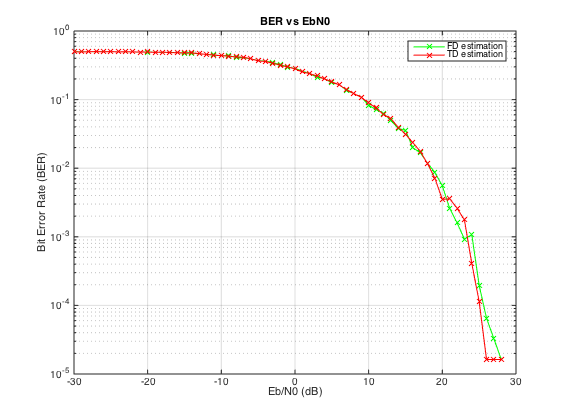
\includegraphics[scale=0.5]{figures/fdvstd_ber.png}
			\vspace{-0.3cm}
			\centering
			\caption{BER performance comparison between FD and TD  channel estimation}
            \label{fig:BER_td}
		\end{minipage}
		\begin{minipage}[t]{0.5\linewidth}
			\centering
			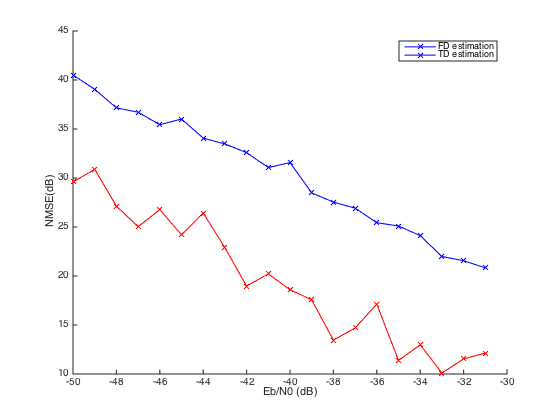
\includegraphics[scale=0.5]{figures/tdvsfd.png}
			\vspace{-0.3cm}
			\centering
			\caption{NMSE comparison between FD and TD channel estimation}
               \label{fig:NMSE_td}
		\end{minipage}
	\end{figure}
    
	\subsection{Synchronization}
	The imperfect local oscillators at the receiver end suffers from both frequency mismatch and time mismatch problem when compared with the transmitter. The block diagram of the synchronization problems are demonstrated in Fig. \ref{fig:sync_intro}. In this section, we will introduce the frequency mismatch and time mismatch problem receptively and their solutions in our simulation.
	
	\begin{figure}[h]
		\centering
		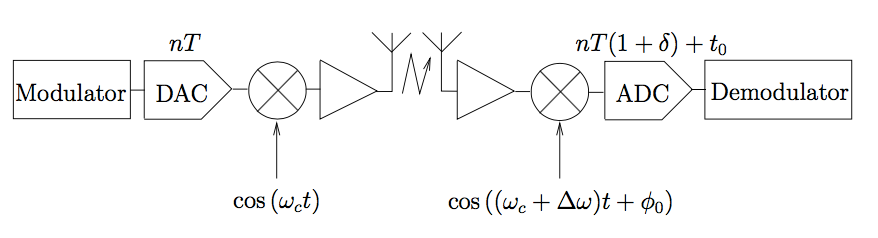
\includegraphics[scale=0.5]{figures/Sync_challenges.png}
		\vspace{-0.2cm}
		\centering
		\caption{Synchronization challenges}
		\label{fig:sync_intro}
	\end{figure}
	
	\subsubsection{Frequency Synchronization}
	Frequency mismatch includes both carrier phase shift $\phi_0$ and the carrier frequency offset $\Delta \omega$. With the presence of the mismatch, the received signal at sub-carrier $p$ is showed in following equations:
	
	\begin{align} 
		\begin{split}
			r_{p} = \sum_{q=-Q/2}^{Q/2-1} I_q^F h^f_q \gamma^0_q \gamma_{p,q} + z_p^F 
		\end{split}
		\label{eq:recev_CFO}
	\end{align}
	
	From Eq. \ref{eq:recev_CFO}, we could find the effect of CFO includes: (i) a phase rotation $\angle (\gamma_q^0)$; (ii) a signal amplitude distortion $|\gamma^0_p|$; (iii) Interference of each carrier on the symbols located on its neighbouring $\gamma_{p,q}$ carriers.
	
	The synchronization is carried out in two steps:
	\begin{itemize}
		\item \textbf{CFO acquisition based on preambles}: A rough estimate of the CFO is obtained during the acquisition phase. The resulting estimate is used to remove most of the CFO from the overall frame. The implementation is quite straight forward, taking two identical preambles, and average the phase shift between them to get the CFO estimation $\hat{\phi}$. Compensation is simply multiplying $e^{-j\hat{\phi}}$ in time domain.
        
        The unambiguous CFO range for preamble detecting is $[-\frac{1}{2NT}, \frac{1}{2NT}]$, in which $N$ is the length of the preamble, and T is the sample time. \textbf{In practice, there is often two stage of preamble acquisition, the first stage with a small $N$, which provide a wider range of detection, then follows a finer detection on a larger $N$.}
        
        It worth mentioning that the CFO acquisition from the preamble is quite rough, especially with the presence of the noise. Fig. \ref{fig:CompFA} shows that even with CFO acquisition from preamble, the BER is still high and unstable.
		
		\item \textbf{Phase tracking based on pilot sub-carriers}: At the output of the acquisition, there remains an error on the carrier frequency (mostly due to the noise). It generates a phase shift growing with the time, that needs to be corrected using phase tracking. Frequency tracking is carried each different data block. In our simulation we choose 4 sub-carriers (-21, -7, 7 and 21) serving as pilots. Phase shifting is constantly estimated in each block by this four pilot sub-carriers and corrected block-wise. Compare Fig. \ref{fig:CompFA} and Fig.\ref{fig:CompFAtotal}, we can observe that the phase tracking enhance the performance significantly. And the tracking is independently carried out for each block.
		
	\end{itemize}
	
	\vspace*{+5mm}
    	\begin{figure}[h]
		\begin{minipage}[t]{0.5\linewidth}
			\centering
			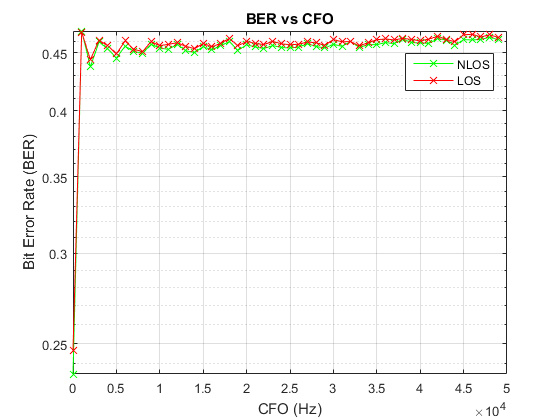
\includegraphics[scale=0.5]{figures/BERvsCFO.png}
			\centering
			\caption{BER vs CFO without frequency acquisition}
            \label{fig:BERvsCFO}
		\end{minipage}
		\begin{minipage}[t]{0.5\linewidth}
			\centering
			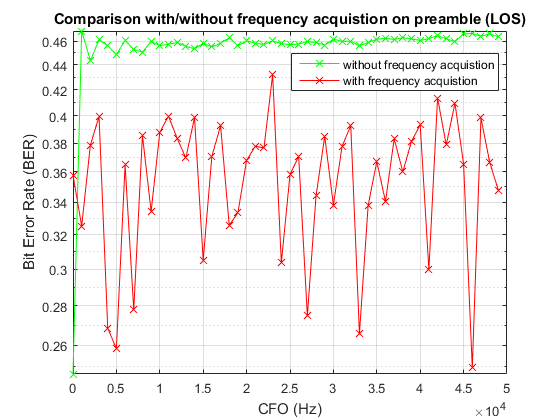
\includegraphics[scale=0.5]{figures/CompFA.png}
			\centering
			\caption{Comparison with/without frequency acquisition based on preamble in LOS case}
            \label{fig:CompFA}
		\end{minipage}
	\end{figure}
    
	\noindent\fbox{%
		\parbox{\textwidth}{%
			\paragraph{Discussions}
			\begin{itemize}
				\item Add the carrier frequency offset to the simulation and evaluate its impact and implement the frequency acquisition;
				\subitem As shown in the Fig. \ref{fig:BERvsCFO}, in NLOS and LOS cases, BER increases drastically after CFO applied and goes up little by little with increase of CFO. This is due to the fact that CFO introduces progressive phase rotation in our model. Frequency acquisition will be applied afterwards to solve this problem.   
				\item Assess its performance and show by simulation that the overall data frame can be decoded in the presence of CFO (which CFO range can be corrected?)
				\subitem We can see from Fig. \ref{fig:CompFA}, after applying frequency acquisition based on preamble, BER value for different CFO is lower indicating that we get better result. The way to do it is described above and we can see that indeed we remove most of CFO in our data. The unambiguous CFO range for preamble detecting is $[-\frac{1}{2NT}, \frac{1}{2NT}]$, and in our model it's $[-156250 Hz, 156250 Hz]$.In order to remove all CFO we use pilots in our data.
				
				\item Replace a few symbols with pilots within the data blocks and implement the frequency tracking.
				\subitem As said before, there are still some errors left on carrier frequency after the previous step leads to phase rotation within each received data block, we use 4 sub-carriers as pilots to remove the residual errors. The phase rotation within each data block is estimated by averaging the phase rotation observed on the pilot symbols interleaved within the data and the remaining CFO can be easily compensated. As a result, Fig. \ref{fig:CompFAtotal} shows that CFO is totally removed from the data received with frequency tracking implemented. 
				
			\end{itemize}
		}%
	}
	
        \begin{figure}[h]
		\centering
		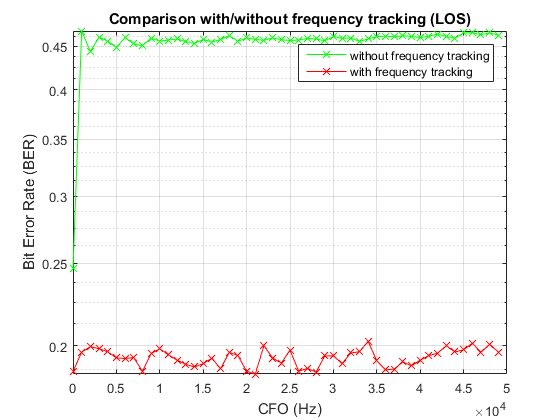
\includegraphics[scale=0.6]{figures/CompFAtotal.png}	
		\centering
		\caption{Comparison with/without frequency tracking in LOS case}
		\label{fig:CompFAtotal}
		\end{figure}
    
	\subsubsection{Time Synchronization}
	
	Time mismatch mainly comes from two factors: sample clock offset(SCO) $\delta \neq 0$ and time shift $t_0 \neq 0$. In the presence of SCO the received signal in frequency domain for sub-carrier $p$ is:
	
		\begin{align} 
		\begin{split}
			r_{p} = \sum_{q=-Q/2}^{Q/2-1} I_q^F h^f_q \gamma^0_q \gamma_{p,q} + z_p^F 
		\end{split}
		\label{eq:recev_SCO}
	\end{align}
	
	where:
    
    	\begin{align}
    	\begin{split}
    	\angle (\gamma_q^0) &\vcentcolon= (\frac{2 \pi t_0}{Q T}-\frac{\pi \delta}{Q}) q \approx \frac{2 \pi t_0}{QT} q  \\
        |\gamma^0_p| &\vcentcolon= \frac{1}{Q} \frac{sin(\pi q \delta)}{sin(\frac{\pi q \delta}{Q})}  \\
        \gamma_{p,q} &\vcentcolon= \frac{(-1)^(q-p) \cdot e^{-j\frac{\pi (q-p)}{Q}}}{cos(\frac{\pi (q-p)}{Q}) + (tan(\frac{\pi q \delta}{Q}))^{-1} sin(\frac{\pi (q-p)}{Q})}
    	\end{split}
    	\end{align}
	
	From the Eq. \ref{eq:recev_SCO}, we could observe that the SCO influence on the receiver includes 3 aspects basically same as CFO, except that the signal amplitude distortion is dependent on the carrier. 
	
	Basically, there are two methods to detect the SCO, namely based on a known preamble and a repetitive preamble. For a known preamble, cross-correlating is calculated with $O(n^2)$ complexity. In this project, we use the repetitive preambles, carrying out the auto-correlation to estimate the time shift. It can be formulated as following:
    
    \begin{align} 
		\begin{split}
			\hat{n} = \max_n p (r_{n+N} | r_n, x_{n+N} = x_n)
		\end{split}
		\label{eq:SCO_auto}
	\end{align}
    
    in which $r_{n+N}$ is the second preamble when the preamble length is $N$, $x_n$ is the symbol located at $n$ in the preamble. The estimation of the time-of-arrival can be done as following:
    
    \begin{align} 
		\begin{split}
			\hat{n} = \max_n \frac{|A_n|}{\sum_{l=0}^{2N-1} |r_{n+l}|^2}
		\end{split}
		\label{eq:SCO_final}
	\end{align}

	\begin{figure}[h]
		\begin{minipage}[t]{0.5\linewidth}
			\centering
			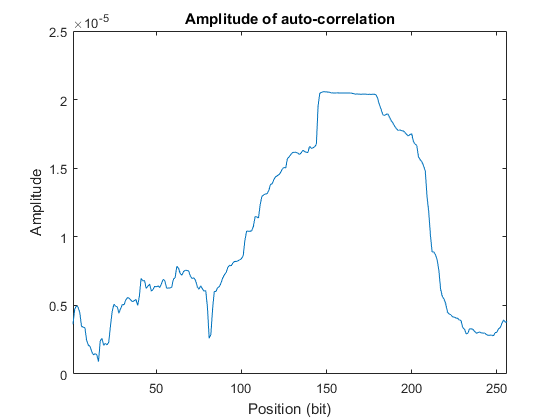
\includegraphics[scale=0.5]{figures/Amp_auto.png}
			\centering
			\caption{Amplitude of correlation}
            \label{fig:Amp_corr}
		\end{minipage}
		\begin{minipage}[t]{0.5\linewidth}
			\centering
			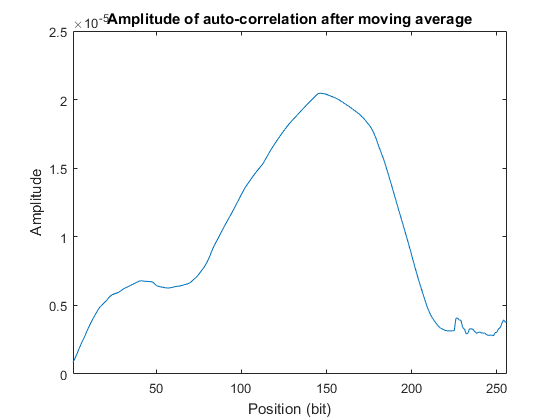
\includegraphics[scale=0.5]{figures/Amp_automean.png}
			\centering
			\caption{Amplitude of correlation with moving mean}
            \label{fig:Amp_corrmean}
		\end{minipage}
	\end{figure}

    in which, $A_n$ is the auto-correlation of the received signal at time $n$ with a replica at time $n+N$. Fig. shows the auto-correlation between two identical preambles in our simulation.

	\vspace*{+5mm}
	
    \begin{figure}[h]
		\centering
		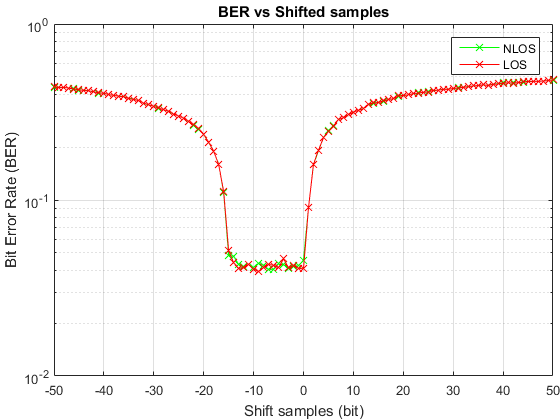
\includegraphics[scale=0.6]{figures/BERvsshiftedNoTA.png}	
		\centering
		\caption{BER vs shifted samples without time acquisition}
		\label{fig:BERvsshiftedNoTA}
		\end{figure}
        
    \begin{figure}[h]
		\begin{minipage}[t]{0.5\linewidth}
			\centering
			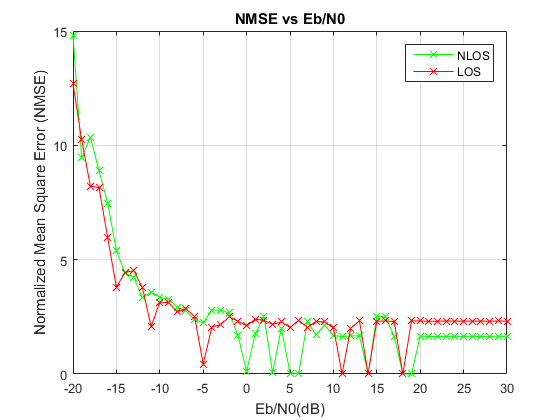
\includegraphics[scale=0.5]{figures/NMSEvsEbN0.png}
			\centering
			\caption{NMSE vs Eb/N0}
            \label{fig:NMSETA}
		\end{minipage}
		\begin{minipage}[t]{0.5\linewidth}
			\centering
			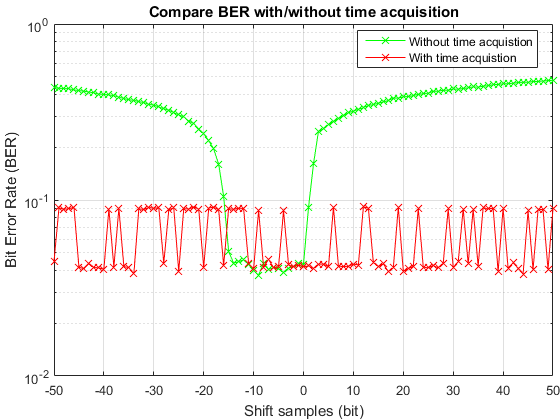
\includegraphics[scale=0.5]{figures/compareBER.png}
			\centering
			\caption{Comparison of BER with/without time acquisition}
            \label{fig:compareBER}
		\end{minipage}
	\end{figure}
    
    \clearpage
    
	\noindent\fbox{%
		\parbox{\textwidth}{%
			\paragraph{Discussions}
			\begin{itemize}
				\item Add the uncertainty on the time-of-arrival to the simulation; Evaluate the impact of an error on the time of arrival estimation;
				\subitem The Time of Arrival(ToA) mismatch influence is showed in Fig \ref{fig:BERvsshiftedNoTA}. As can be seen from the figure that when there are shifted samples appeared in the transmitted signal without time acquisition in the receiver, BER value increases drastically compared to no error on TOA case. Also we can see that there is a plateau of low level BER with a length of CP, this indicates that if TOA is estimated a little bit late we still have a result similar to no error situation. 
                
				\item Implement the time acquisition. The cyclic prefix introduces an unwanted effect. Explain this
effect and carefully deal with it;
				\subitem As can be seen in Fig. \ref{fig:Amp_corr} there is a plateau with the length of CP of preamble. Since that CP of preamble is replica of data in preamble, so that the correlation between CP and preamble is very high. To deal with this effect, moving mean with length of plateau is applied, as shown in Fig. \ref{fig:Amp_corrmean} we can see a peak appears after this, this is the location of the center of CP plus the half of the length of moving window used in moving mean. In this way, we can get the number of shifted data.
                
				\item Evaluate the accuracy achieved on the time-of-arrival estimate (Root Mean Square Error of the
estimate as a function of the signal to noise ratio). Does the time-of-arrival estimation impact the BER performance?
				\subitem The accuracy achieved is shown in Fig. \ref{fig:NMSETA}, NMSE is decreasing with increase of Eb/N0 which is reasonable since with high Eb/N0 noise will have less influence on signal and it will help receiver to estimate the channel. In the Fig. \ref{fig:compareBER} we can see that after applying time acquisition, BER value is much lower than without time acquisition case no matter how much samples are shifted. Also we can see some peaks appearing in red line, this is caused by the noise added on data.
                
			\end{itemize}
		}%
	}
    
    \vspace*{+5mm}	
	
    The SIMO communication system in this simulation refers to the system with single transmitter and multiple receiver. Exactly the same signal is transmitted, and different signal is received due to the different spatial location of the receiving antenna. Eq. \ref{eq:SIMO_intor} shows the formula for the SIMO system we simulated:
     \begin{align} 
		\begin{split}
			y = \textbf{H}x + n
		\end{split}
		\label{eq:SIMO_intor}
	\end{align}
    
    in which $y$ and $\textbf{H}$ are both vectors, indicating the received signal and transfer functions from different channels.
    
	\subsection{SIMO channel}
    
    \paragraph{Beamforming} To model the different incident waves from different angular directions. We employ the 3D beamformer function $B_i(\theta, \phi)$ to formulate the directional delay. Then the amplitude of each incident wave can be expressed by following:
    \begin{align} 
		\begin{split}
			a_n(\theta, \phi) = \frac{\sum_i \hat{h_i}(n) \cdot B_i^*(\theta, \phi)}{\sum_i | B_i(\theta, \phi) |^2}
		\end{split}
		\label{eq:beamforming}
	\end{align}
    
    We choose to scan the $\phi$ in the range of $[0, \pi]$ with 20 points, and $\theta$ in the range of $[-\pi, \pi]$ with 40 points. With the lab measurement as input, we get the following result for NLOS and LOS scene respectively:
    
    \begin{figure}[h]
		\centering
		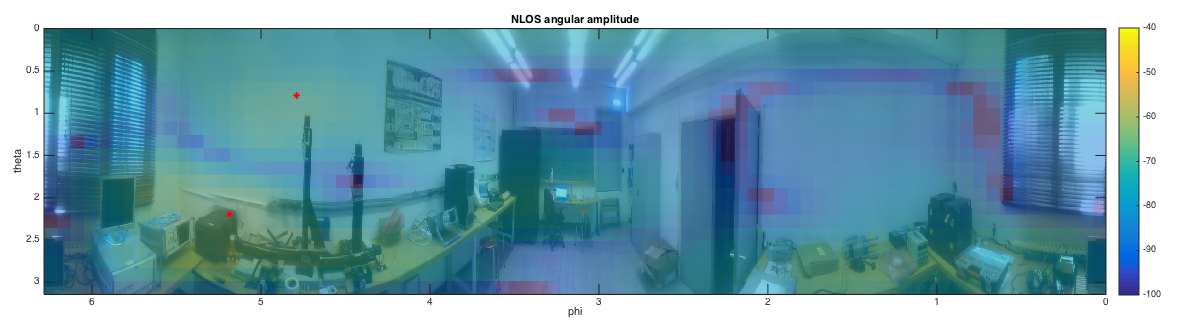
\includegraphics[scale=0.4]{figures/NLOS_angular.png}
		\vspace{-0.2cm}
		\centering
		\caption{NLOS angular amplitude distribution}
		\label{fig:angular_nlos}
	\end{figure}
    
    \begin{figure}[h]
		\centering
		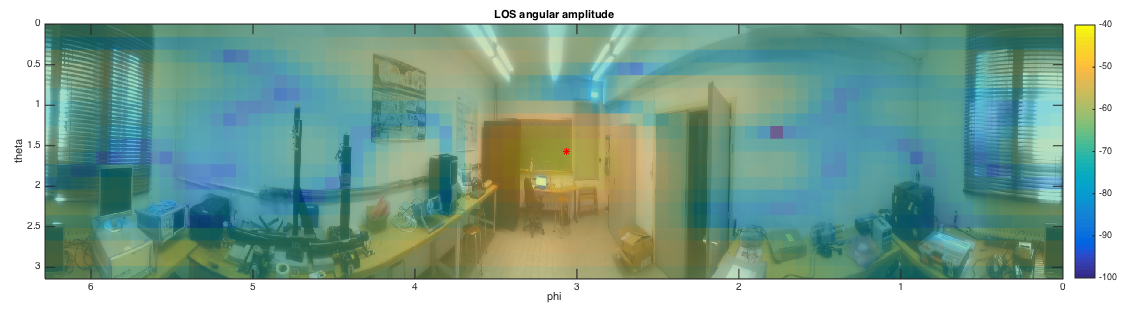
\includegraphics[scale=0.42]{figures/LOS_angular.png}
		\vspace{-0.2cm}
		\centering
		\caption{LOS angular amplitude distribution}
		\label{fig:angular_los}
	\end{figure}
	
    \paragraph{Spatial Correlation}
    Spatial correlation is an important parameter for the channel model. As the environment around the transmitter and the receiver is the same, we assume the channel is reciprocal. Take the spacial correlation along z-axis as an example. Eq. formulate the spatial correlation under the uncorrelated scattering assumption:
    
    \begin{align} 
		\begin{split}
			R(\Delta z) = \sum_{i=1}^{N_u} |a(u_i)|^2 e^{ju_i\Delta z}
		\end{split}
		\label{eq:spatialCorr}
	\end{align}
    
    \begin{figure}[ht]
		\begin{minipage}[t]{0.5\linewidth}
			\centering
			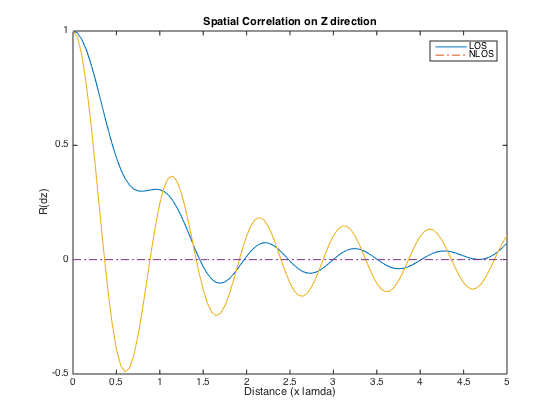
\includegraphics[scale=0.4]{figures/wb_spc_Z.png}
			\vspace{-0.3cm}
			\centering
			\caption{spatial correlation along Z-axis (Wideband, tap=1)}
            \label{fig:wb_spc_z}
		\end{minipage}
		\begin{minipage}[t]{0.5\linewidth}
			\centering
			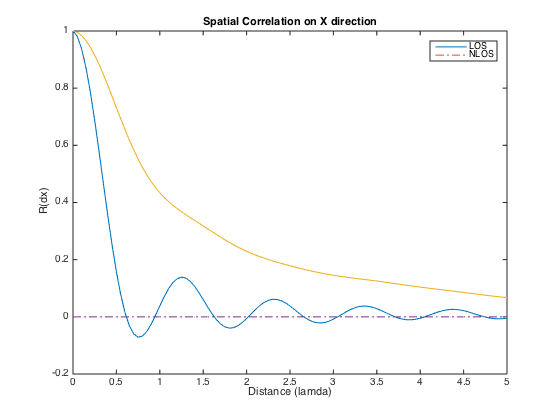
\includegraphics[scale=0.4]{figures/wb_spc_X.png}
			\vspace{-0.3cm}
			\centering
			\caption{spatial correlation along X-axis (Wideband, tap=1)}
            \label{fig:wb_spc_x}
		\end{minipage}
    \end{figure}
    
    \begin{figure}[ht]
		\begin{minipage}[t]{0.5\linewidth}
			\centering
			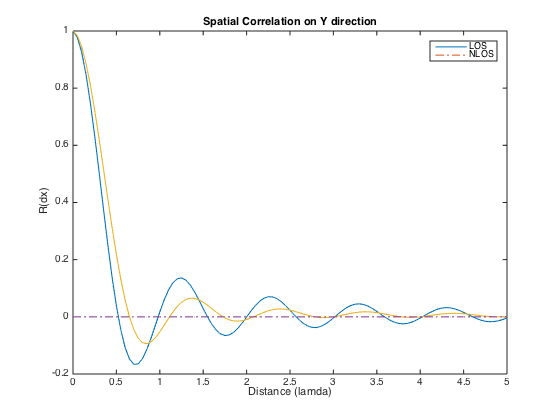
\includegraphics[scale=0.4]{figures/wb_spc_Y.png}
			\vspace{-0.3cm}
			\centering
			\caption{spatial correlation along Y-axis (Wideband, tap=1)}
            \label{fig:wb_spc_y}
		\end{minipage}
		\begin{minipage}[t]{0.5\linewidth}
			\centering
			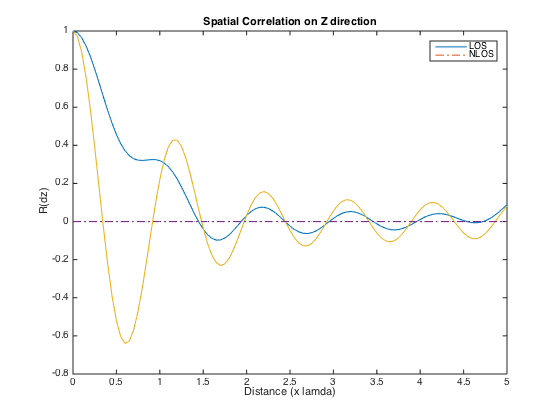
\includegraphics[scale=0.4]{figures/nb_spc_Z.png}
			\vspace{-0.3cm}
			\centering
			\caption{spatial correlation along Z-axis (narrowband)}
            \label{fig:nb_spc_z}
		\end{minipage}
    \end{figure}
    
    \begin{figure}[ht]
		\begin{minipage}[t]{0.5\linewidth}
			\centering
			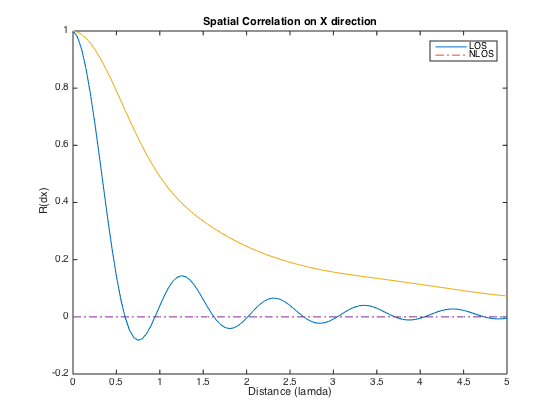
\includegraphics[scale=0.4]{figures/nb_spc_X.png}
			\vspace{-0.3cm}
			\centering
			\caption{spatial correlation along X-axis (narrowband)}
            \label{fig:nb_spc_x}
		\end{minipage}
		\begin{minipage}[t]{0.5\linewidth}
			\centering
			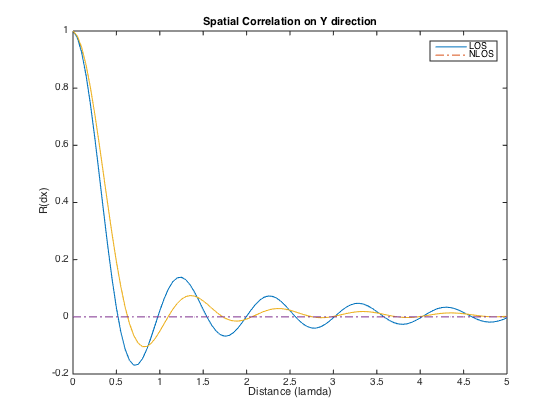
\includegraphics[scale=0.4]{figures/nb_spc_Y.png}
			\vspace{-0.3cm}
			\centering
			\caption{spatial correlation along Y-axis (narrowband)}
            \label{fig:nb_spc_y}
		\end{minipage}
    \end{figure}
    
    \vspace*{+5mm}
	
	\noindent\fbox{%
		\parbox{\textwidth}{%
			\paragraph{Discussions}
			\begin{itemize}
				\item Explain the beamforming method and deduce by using beamforming the angular spectrum of the MPCs for each tap;
				\subitem The beamforming method is explained in Section 4.4, while the angular amplitude distribution for the measurement is demonstrated in Fig. \ref{fig:angular_nlos} and Fig. \ref{fig:angular_los}.
                %TODO: adding the figure showing the TOA influence
				\item Build a physical model of the channel for each tap based on beamforming;
				\subitem 
				\item Study the spatial correlation of the channel model you built as a function of distance between
antennas, for the three directions - x, y, z - in narrowband and wideband. Compare to Clarke’s
model.
				\subitem The spatial correlation is calculated  along x,y,z axis. Fig. \ref{fig:wb_spc_z} - \ref{fig:wb_spc_y} shows the correlation for the first tap.  Fig. \ref{fig:nb_spc_z} shows  the spatial correlation along the z-axis for narrowband model. Comparing with Fig. \ref{fig:wb_spc_z} and Fig. \ref{fig:nb_spc_z}, we could observe few difference between narrowband and wideband model. We can also observe from the figures that all the spatial correlations are coherent with the Clark's model following a Bessel function along the -x, y, z- axis. And the coherence distance occurs at around half of the wavelength of the signal.
                
			\end{itemize}
		}%
	}
    
	\subsection{Communication with multiple antenna receiver}
	
    In this project, a multiple antennas receiver is deployed at the receiver. The system employ the conventional maximum ration combining (MRC) technique to each sub-carrier independently. It worth mentioning that the CFO and time of arrival is the same for each received signal as all the antenna is sharing the same local oscillator .
    
    \begin{figure}[h]
		\centering
		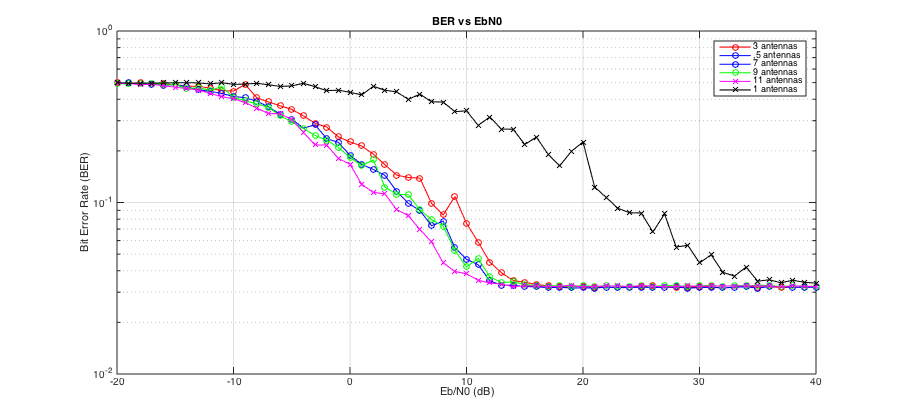
\includegraphics[scale=0.5]{figures/num_antennas.png}
		\centering
		\caption{Compare the BER performance between different number of receiver antennas}
		\label{fig:lab7_nantennas}
	\end{figure}
    
    \vspace*{+5mm}
	
	\noindent\fbox{%
		\parbox{\textwidth}{%
			\paragraph{Discussions}
			\begin{itemize}
				\item Update the communication chain to implement the SIMO system on MATLAB with the new channel model and assess the bit error rate performance as a function of the number of antennas;
				\subitem 
                In Fig. \ref{fig:lab7_nantennas} we can observe that with the increasing numbers of the antennas, the BER vs EbN0 performance is improving as well. Significant improving can be observed when applying 3 antennas instead of only one receiver antenna. With the increasing of number of antennas, the benefit is increasing more less and less significantly.
				\item Discuss the interest of MRC compared to a simple symbol combination;
				\subitem 
				\item Illustrate the benefit of spatial diversity on the obtained BER curves.
				\subitem In Fig. \ref{fig:lab7_nantennas}, we showed the benefit of employing the SIMO over the SISO communication system. From the BER graph, we can observe that SIMO system over-perform the SISO system significantly. 
			\end{itemize}
		}%
	}
    
	\section{Conclusion}
	In this project, we finished a MATLAB based simulation for a wireless communication system. The system is based on the IEEE 802.11n standard, and features OFDM. Wireless communication channel model is also extracted based on real-life measurement, the channel is characterized and extracted statistically on both Line-of-Sight(LOS) and Non-LOS scene. It is employed in the simulation to give a more realistic channel function. Details concerning the OFDM, synchronization and SIMO are introduced and discussed in this report. The benefit of employing multiple receiver is demonstrated in the simulation by comparing with the SISO system. 
    
	\paragraph{Sample availability} The fore-mentioned simulation is available on github with following link. Please contact the authors for further question. 
    
    https://github.com/Walkerlikesfish/DigitalCommunication.git
	
\end{document}